% HMC Math dept HW template example
% v0.04 by Eric J. Malm, 10 Mar 2005
\documentclass[12pt,letterpaper,boxed,cm]{hmcpset}

% set 1-inch margins in the document
\usepackage[margin=1in]{geometry}
\usepackage{mathtools}
\usepackage{mathrsfs}
% include this if you want to import graphics files with /includegraphics
\usepackage{graphicx}
\usepackage{cases}
\usepackage{hyperref}
\usepackage{siunitx}
\usepackage{tikz}
\usetikzlibrary{arrows}

% info for header block in upper right hand corner
\name{Name: ~~~~~~~~~~~~~~~~~~~~~~}
\class{Physics 51}
\assignment{Homework \#4}
\duedate{September 12, 2016}

\newcommand{\ev}[2]{\Big|_{#1}^{#2}}
\newcommand{\evv}[2]{\Big|_{#1}^{#2}}
\newcommand{\set}[1]{\left\{#1\right\}}
\newcommand{\s}[1]{\sqrt{#1}}
\newcommand{\f}[2]{\frac{#1}{#2}}
\newcommand{\p}[2]{\frac{\partial #1}{\partial #2}}
\providecommand{\t}[1]{\text{#1}}
\providecommand{\span}[1]{\text{span}\left(#1\right)}
\providecommand{\set}[1]{\left\{#1\right\}}
\providecommand{\l}[0]{\left}
\providecommand{\r}[0]{\right}
\newcommand{\m}[1]{\begin{matrix}#1\end{matrix}}
\newcommand{\bm}[1]{\begin{bmatrix}#1\end{bmatrix}}
\renewcommand{\bf}[1]{\mathbf{#1}}
\newcommand{\pn}[1]{\left( #1 \right)}
\newcommand{\abs}[1]{\left| #1 \right|}
\newcommand{\bk}[1]{\left[ #1 \right]}
\newcommand{\cis}[1]{\pn{\cos\pn{#1} + i\sin\pn{#1}}}
\newcommand{\cisi}[1]{\pn{\cos\pn{#1} - i\sin\pn{#1}}}
\renewcommand{\Im}[1]{\text{Im}\pn{#1}}
\renewcommand{\Re}[1]{\text{Re}\pn{#1}}

\makeatletter
\renewcommand*\env@matrix[1][*\c@MaxMatrixCols c]{%
  \hskip -\arraycolsep
  \let\@ifnextchar\new@ifnextchar
  \array{#1}}
\makeatother
\begin{document}
\problemlist{27-P8, 27-P16, 27-P17, SUP1*}

\begin{problem}[27-P8]
Figure 35 shows a section through two long thin concentric cylinders of radii $a$ and $b$. The cylinders carry equal and opposite charges per unit length $\lambda$. Using Gauss' Law, prove 
\begin{enumerate}
	\item[(a)] that $E = 0$ for $r < a$ and
	\item[(b)] that between the cylinders $E$ is given by
\[
	E = \f{1}{2\pi\epsilon_0} \f{\lambda}{r}.
\]
\end{enumerate}
\begin{center}
	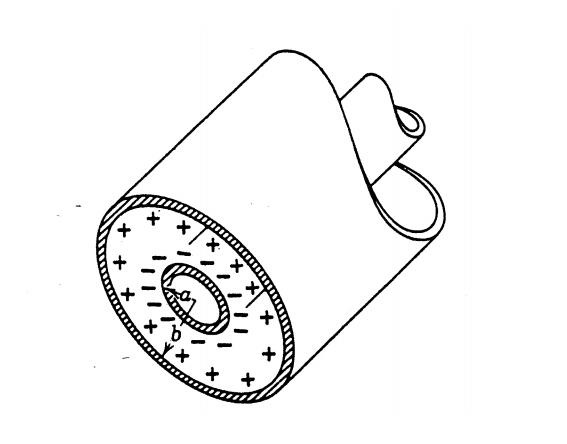
\includegraphics[scale=0.7]{01.png}
\end{center}
\end{problem}
\begin{solution}
\end{solution}
\newpage

\begin{problem}[27-P16]
A plane slab of thickness $d$ has a uniform volume charge density $\rho$. Find the magnitude of the electric field at all points in space both (a) inside and (b) outside the slab, in terms of $x$, the distance measured from the median plane of the slab.
\end{problem}
\begin{solution}
\end{solution}
\newpage

\begin{problem}[27-P17]
A solid nonconducting sphere of radius $R$ carries a nonuniform charge distribution, with charge density $\rho = \rho_s r/R$, where $\rho_s$ is a constant and $r$ is the distance from the center of the sphere. Show that
\begin{enumerate}
	\item[(a)] the total cnharge on the sphere is $Q = \pi\rho_sR^3$ and
	\item[(b)] the electric field inside the sphere is given by
\[
	E = \f{1}{4\pi\epsilon_0} \f{Q}{R^4} r^2.
\]
\end{enumerate}
\end{problem}
\begin{solution}
\end{solution}
\newpage

\begin{problem}[SUP1*]
A nonconducting hemispherical cup of inner radius $R$ has a total charge $q$ spread uniformly over its inner surface. Find the electric field at the center of curvature. (Hint: Consider the cucp as a stack of rings.)
\end{problem}
\begin{solution}
\end{solution}
\end{document}
